\chapter{Objective Assessment}
\label{chap:objective}

\section{Application requirements}
For building the application, Mobai was very open in terms of how we wanted to build it. They only came up with a few requirements:
\begin{itemize}
    \item The application should be able to be containerized and ran independently in a docker container.
    \item The application should have a front- and backend functionality.
    \item The backend should be built in a simple way to easily add new FIQM's into the system.
\end{itemize}
Other than this, Mobai gave us no restrictions on what software we had to use to develop the application. They gave us a vocal introduction on how they wanted the application to work, and from there, we started to create the main functional requirements. It is important to mention that Mobai was quite open for suggestions regarding the functionality and that new functional requirements were formed during the development process, both from Mobai's part and from our suggestions. This means that some functional requirements were not clear to us before the middle of the development process, and we had to take that into consideration when choosing our development method. It wasn't before the middle of march we got a clear understanding of exactly what requirements Mobai had for the application and we could create specific functional requirements for the whole application. We have chosen to display all the functional requirements in the form of use cases and a use case diagram. Note that the functional requirements differ in terms of frontend and backend functionality, and that the backend functionality should work independently from the frontend:         

\newpage

\section{Use case}
We have created a use case diagram to show the core functionality and activities within the application. The diagram was build from the perspective of the user (described in Section \ref{sec:TargetGroups}) which are employees at Mobai. The cases differ in complexity where running all metrics would be the most challenging. That is because it includes running every metric and providing scores for each image. 

\begin{figure}[h]
    \centering
    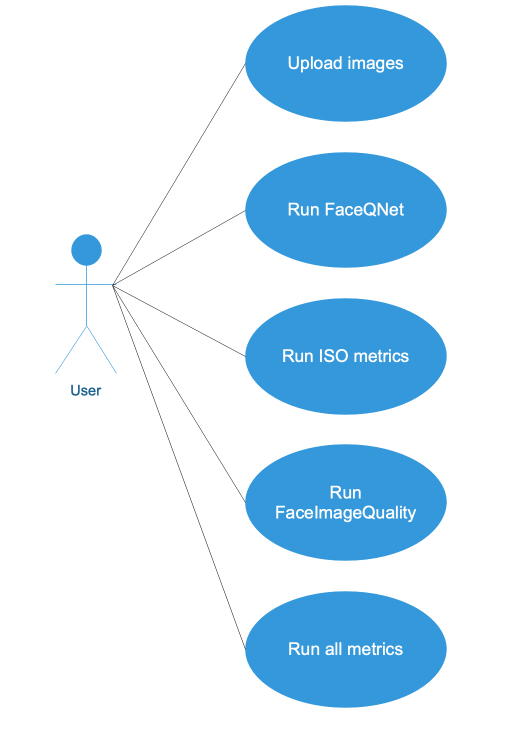
\includegraphics[scale = 0.4]{figures/UseCaseDiagram.png}
    \caption{Use case diagram}
    \label{fig:UseCase}
\end{figure}

\begin{table}[h]
\centering
\resizebox{\textwidth}{!}{%
\begin{tabular}{|p{12cm}|} 
\hline
\textbf{Use case:} Upload images\\
\textbf{Actor:} User \\
\textbf{Goal:} Upload selected images \\
\textbf{Description:} The user can select which images he would like to upload to the application. Images will only be stored in the application for that session. \\ \hline
\end{tabular}%
}
\end{table}

\newpage

\begin{table}[h]
\centering
\resizebox{\textwidth}{!}{%
\begin{tabular}{|p{12cm}|} 
\hline
\textbf{Use case:} Run ISO metrics\\
\textbf{Actor:} User \\
\textbf{Goal:} Evaluate images with the ISO metric \\
\textbf{Description:} After uploading selected images, the user would push ''Run ISO metrics'' to assess the images. The application returns a sheet with quality scores for each facial image. \\ \hline
\end{tabular}%
}
\end{table}

\begin{table}[h]
\centering
\resizebox{\textwidth}{!}{%
\begin{tabular}{|p{12cm}|} 
\hline
\textbf{Use case:} Run FaceQNet\\
\textbf{Actor:} User \\
\textbf{Goal:} Evaluate images with the FaceQNet \\
\textbf{Description:} After uploading selected images, the user would push ''Run FaceQNet'' to assess the images. The application returns a sheet with quality scores for each facial image. \\ \hline
\end{tabular}%
}
\end{table}

\begin{table}[h]
\centering
\resizebox{\textwidth}{!}{%
\begin{tabular}{|p{12cm}|} 
\hline
\textbf{Use case:} Run FaceImageQuality\\
\textbf{Actor:} User \\
\textbf{Goal:} Evaluate images with the FaceImageQuality \\
\textbf{Description:} After uploading selected images, the user would push ''Run FaceImageQuality'' to assess the images. The application returns a sheet with quality scores for each facial image. \\ \hline
\end{tabular}%
}
\end{table}

\newpage

\begin{table}[h]
\centering
\resizebox{\textwidth}{!}{%
\begin{tabular}{|l|p{9cm}|} 
\hline
\textbf{Case} & Run all metrics  \\ \hline
\textbf{Description} & The user runs all metrics in the applications which returns scores for every image.      \\ \hline
\textbf{Basic Flow} &   \begin{enumerate}
    \item The user pushes the upload images button.
    \item The user navigates to select wanted images to perform the metrics on.
    \item After uploading images, the user presses ''Run all metrics''
    \item The program returns a sheet with quality scores of the selected images
\end{enumerate}     \\ \hline
\textbf{Alternative} &  The user runs all metrics without uploading any images
            \begin{enumerate}
                \item The application displays an error and asks the user to upload images.
            \end{enumerate}
The user presses reset before running the metrics 
            \begin{enumerate}
                \item Uploading images again is necessary
            \end{enumerate}
                    \\  \hline
\textbf{Pre-condidtion} & The application is running. \\ \hline
\textbf{Post-condition} &  Images that are being evaluated are uploaded. \\ \hline
\end{tabular}%
}
\caption{High level use case for ''Run all metrics''}
\end{table}


\section{Choice of front- and backend}
When choosing development software, we had to take some considerations. First, both backend and frontend software should not be time consuming to master, given that the project consisted of coding and research. Second, it should be uncomplicated to integrate the released FIQMs with the backend as well as creating an intelligible user interface. 

\subsection*{Backend}
The two FIQMs FaceQNet and ISO metrics were written in python. Since we were experienced with python and operated with it in courses throughout the bachelor program, it was natural to choose a python framework for the backend. With a dozen of possible web frameworks, we needed to select a framework which suited our needs in terms of scalability, performance and ease of use. In the end, the choices were between Django and Flask. 


\begin{table}[h]
\centering
\resizebox{\textwidth}{!}{%
\begin{tabular}{|l|p{9cm}|} 
\hline
\textbf{Framework} & Django  \\ \hline
\textbf{Advantages} &  Django is a fast framework, making the development process for the developers to increase. It has as high level of scaliability to the users. This feature is the reason many leading websites depend on Django to fulfill their high operational requirements. The framework includes several prebuild development features as user authentication, sitemaps, content administration etc. It has excellent security, preventing the users from several security issues. Django is very flexible as it can be used to create a widely specter of application types. Some of these are social networking such as Instagram or content management systems such as Wagtail \cite{DjangoAdvantages}.     \\ \hline
\textbf{Disadvantages} & First of all, Django has a steep learning curve. Even though it its written in python, it takes a long time for developers to get the hang of it. The framework is considered one of the hardest to master. Django is more suitable for large scale applications rather than smaller products with fewer features and requirements. The unique functionalities within Django can be confusing for developers working with a small project. Djangos' monolithic architecture has a small number of dependencies which make it challenging to use. It does not facilitate developers to utilize python packages and tools, but focuses on code-oriented programming. Django can not provide fast development in terms on requests. Only one request at the time can be fulfilled, meaning it is unable to handle multiple requests concurrently\cite{DjangoDisadvantages}.         \\ \hline
\end{tabular}%
}
\caption{Pros and cons with Django}
\end{table}

\begin{table}[h]
\centering
\resizebox{\textwidth}{!}{%
\begin{tabular}{|l|p{9cm}|}
\hline
\textbf{Framework} & Flask  \\ \hline
\textbf{Advantages} & For programmers with experience in python, it is easy adaptable to work with Flask. This micro framework is simple to manage as there are few standards. Flasks' modular nature let developers instantly create servers and applications, which are distributed across comprehensive networks with certain purposes. It is pliable, meaning that components within the framework are easy to modify, because it is simple to configure. Given that Flask is a micro framework, it has less abstraction layers between the users and the database, cache and requests. This design provide users high level of performance.\cite{DjangoAdvantages}  \\ \hline
\textbf{Disadvantages} & As many beginner web developers tend to use the Flask framework, resulting in low quality code and possibly a bad application. Flask has singular source, meaning that is handles requests in turns. With multiple requests, it could be time consuming to handle the requests. The use of modules in Flask raises security issues. It would be bad if a module contained spiteful data.             \\ \hline
\end{tabular}%
}
\caption{Pros and cons with Flask}
\end{table}

Initially, we started the backend development process using Django. This was mainly because the team working with backend had learned about the framework in an earlier course of the bachelor program. However, we eventually concluded not to use Django for the backend. Given some knowledge in the framework, we had not actually developed anything with it. Since Django did not provide the usage of python packages or tools, it would be more time consuming to code the application. The steep learning curve provided by the framework would make the development process even more time consuming. Our project differed in working tasks, by not only have a coding task, made the application smaller in terms of features and requirements. Django was more suitable for larger applications, making the decision of not using the framework clearer. We ended up using Flask for the backend. Immediately after installing the framework, the development productivity increased rapidly. Our python experience was easily adaptable to Flask which made it simple to make a deployable application and integrate FIQMs to the program. 

\subsection*{Frontend}

\subsection*{Containerization}
One of the few requirements given by Mobai was to deploy the application in a container. With such a containerization \cite{Containerization}, it provided us a lot of benefits:
\begin{itemize}
    \item A container is independent of the operating system, making it portable between dissimilar platforms. 
    \item Containers are efficient in terms of allowing applications being quickly deployed, patched or scaled. 
    \item Containers consume less system overhead than regular hardware or virtual environment owing to that they do not include operating system images. 
    \item It provides better application development, production cycles and testing as containers supports an agile workflow.
    \item Having the application separated into different containers will improve security. 
\end{itemize}


